\documentclass[11pt,a4paper]{article}
%\documentclass[10pt,twocolumn]{article}

\usepackage{Autres} %% cibler doc/modules/
\setlength{\columnsep}{1cm}


%\onecolumn
\begin{document}
  \fairetitre{Amélioration de la réactivité des réseaux pair à pair pour les MMOGs}{Les différentes idées d'amélioration}{Xavier Joudiou}{Sergey Legtchenko \& Sébastien Monnet}{17/06/10}

\newpage
%\onecolumn
\tableofcontents
\newpage
%\twocolumn

\noindent{\textbf{Résumé}}\\
	\par \textit{Depuis plusieurs années, un nouveau type d'architecture des systèmes est apparu. Il s'agit de l'architecture pair à pair, cette architecture est devenue populaire grâce à des applications de partage de fichiers. Nous allons nous intéresser aux jeux vidéos massivement multijoueur (MMOG pour Massively Multiplayer Online Games) qui sont de plus en plus populaires et qui font ressortir des problèmes que l'architecture pair à pair doit pouvoir corriger. Le problème du passage à l'échelle sera l'un des plus importants à résoudre pour permettre à un grand nombre de joueurs de participer simultanément. Nous verrons comment l'architecture pair à pair peut être une des solutions.\\ 
	 Pour remédier à cela, une solution consiste à remplacer le modèle client/serveur par un réseau logique pair à pair (overlay). Malheureusement, les protocoles pair à pair existants sont trop peu réactifs pour assurer la faible latence nécessaire à ce genre d’applications. Néanmoins, quelques travaux ont déjà été menés pour adresser ce problème. L’idée est d’adapter le voisinage de chaque pair afin que toute l’information dont il aura besoin dans l'avenir se trouve proche de lui dans le réseau. Il est alors nécessaire de correctement évaluer les futurs besoins de chaque pair, et de faire évoluer son voisinage à temps. Dans ce rapport bibliographique, nous allons étudier les mouvements de groupe et ainsi nous pourrons voir si cette piste est exploitable pour l'amélioration de la réactivité des réseaux pair à pair pour les MMOG.}\\


\section{Introduction}
Ce document va récapituler les différentes solutions d'amélioration de la réactivité des réseaux pair à pair pour les MMOG. Il faudra tenir compte de la difficultés et du temps de mise en place de chaque solution, pour choisir la solution qui sera réalisable avant la fin du stage et qui puisse apporter des améliorations non négligeables.
Plusieurs pistes sont envisagées dont celle menant aux mouvements de groupe, que l'on peut aussi retrouver de façon plus précises dans un rapport bibliographique qui lui est dédié.

\newpage
\section{Mise en place d'un cache pour les zones peuplées}
La mise en place d'un cache pour les zones peuplées permettrait d'améliorer la réactivité dans un état (\textbf{W}) qui n'est pas encore améliorée. L'avantage de cette solution, même si l'issue n'est pas certaine, est de s'intéresser à une partie que l'on n'a pas encore fait évoluée. 
\par Le but de cette solution serait de mettre en place un cache qui garderait un certains nombre de nœud qui viennent de sortir de la liste des voisins du nœud. Ainsi comme les mouvements de l'avatar sont désordonnés, il est possible qu'il retourne vers des nœuds qu'il vient de quitter. Sur la figure~\ref{cacheW}, il est possible de se faire une idée de cette solution.
	\begin{figure}[!h]
        \centering
        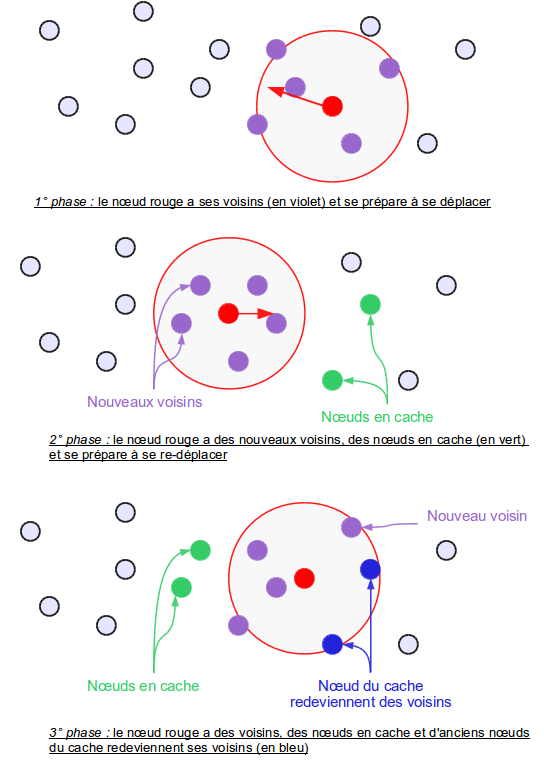
\includegraphics[scale=0.40]{./images/cacheW.png}
        \caption{Exemple de gain possible pour le prefetching}
        \label{cacheW}
        \end{figure} 
\par Sur la figure~\ref{cacheW}, un exemple de l'utilisation du cache est mis en avant. Nous pouvons voir trois phases durant lesquelles un nœud (rouge) va bouger et modifier ses voisins à chaque instant. Les nœuds, qui étaient voisins et qui ne le sont plus à l'instant suivant, sont placés dans le cache. Ainsi lorsque le nœud revient vers eux, ce dernier n'aura pas à refaire une recherche de voisins avec les deux nœuds verts, il aura juste à demander aux nœud verts si ils sont toujours au même endroit, etc.
\par Cette solution pourrait économiser des messages de découverte des voisins dans le cas de changements de direction fréquents. Mais l'efficacité de cette méthode n'est pas sure. 
 
\section{Mécanismes de connaissance des routes entre les Hotspots}
Dans cette solution, nous voudrions permettre que les avatars suivent des routes pour par exemple simuler le contournement d'un obstacle. Il faudrait donc modifier le modèle pour ajouter des obstacles. Il faudrait alors définir des chemins et les conserver dans l'environnement. Cette solution permettrait de simuler un comportement réel, et ainsi d'essayer d'améliorer cette situation.
\par Les modification sur le modèle ne seront peut être pas très simple, il faudrait aléatoirement, comme il a été fait pour les Hotspots, définir des zones où les avatars ne pourraient pas passer ou seraient ralenti. Sur la figure~\ref{trajobstacle}, nous pouvons voir des trajectoires permettant d'éviter l'obstacle. Il faut définir si ces trajectoires se font par apprentissage ou si elles sont données avec l'initialisation de la carte.
	\begin{figure}[!h]
        \centering
        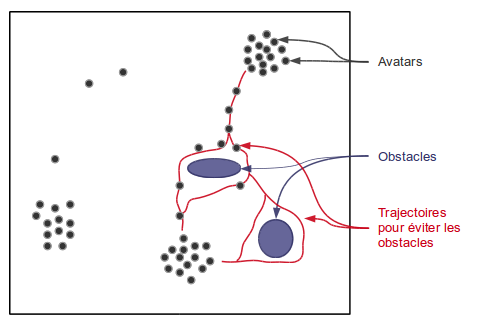
\includegraphics[scale=0.55]{./images/trajobstacle}
        \caption{Exemple de trajectoire d'évitement d'un obstacle}
        \label{trajobstacle}
        \end{figure}

\newpage
\section{Amélioration du prefetch de Blue Banana}
Une des solutions est d'essayer d'améliorer le travail déjà réalisé dans Blue Banana~\cite{191}, l'objectif serait prefetcher plus finement les nœuds. Pour le moment, nous regardons juste les nœuds qui sont dans notre champs de vision (un cône) et qui ne sont ni trop loin, ni trop près. Mais il serait intéressant d'avoir plus d'informations sur les nœuds, comme leur direction ou leur vitesse par exemple. 
\par Actuellement un nœud, qui est dans l'état \textbf{T}(ravelling), va chercher des nœuds qui se trouvent sur la trajectoire probable de l'avatar, tant que son ensemble de voisins n'est pas plein. Ce mécanisme va donc rapatrier des données qui sont à bonne distance (pas trop près à cause des temps de communication), un des risques est de rapatrier des nœuds qui sont inutiles si l'avatar change de direction ou d'état. Ce mécanisme ne va pas non plus observer les différentes propriétés des nœuds (vitesse, direction, état, etc) et dans certains cas, il est possible qu'il rapatrie des nœuds qui viennent vers lui très rapidement et qui ne seront donc pas utiles.
\par L'idée est donc en plus de la distance avec le nœud, il faudrait tester les différentes propriétés. Une solution serait peut être d'essayer de déterminer de façon simpliste les futures positions des nœuds et de tenir compte du couple vitesse/direction, pour mieux rapatrier les données. De plus, il faudrait chercher parmi des nœuds qui peuvent être hors du cône, mais sans trop chercher sinon trop de messages seront émis.
\par  Nous pouvons voir un exemple de l'avantage de cet ajout (voir figure~\ref{prefecthav}), qui pourrait, par exemple, permettre l'ajout du nœud en rouge au lieu du vert.
	\begin{figure}[!h]
        \centering
        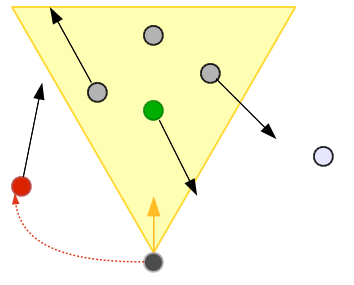
\includegraphics[scale=0.45]{./images/prefetchav.png}
        \caption{Exemple de gain possible pour le prefetching}
        \label{prefetchav}
        \end{figure}

\newpage
\section{Les mouvements de groupe}
Cette partie est décrit de façon plus précise dans le rapport bibliographique qui lui est consacré. Il nous a été possible d'observer, à travers différentes études~\cite{1124834,1124834,1031667}, que les joueurs se déplacent fréquemment en groupe. Ces déplacements se font la plupart du temps entre les joueurs d'un même guilde. Nous pouvons observer sur la figure~\ref{recapstat} qu'en grande majorité les joueurs font partie de groupe, c'est pour cela que cette solution peut être intéressante. 
\par Pour mettre en place cette solution, il faudra refaire un modèle de mobilité qui met en place des déplacements de groupe. Ce travail pourrait prendre plus de temps que les autres solutions car il nécessite un bon nombre de changement dans l'existant.

	\vspace{1cm}
        \begin{figure}[!h]
        \centering
        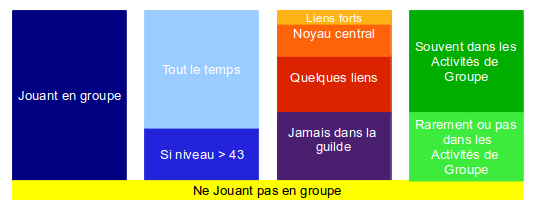
\includegraphics[scale=0.65]{./images/recapstat.png}
        \caption{Schéma récapitulatif des activités de groupe}
        \label{recapstat}
        \end{figure}
\par L'utilisation des mouvements de groupe pourraient nous permettre de réorganiser le prefetching des données, et ne plus considéré les nœuds indépendamment mais comme formant un groupe. Ces groupes vont devoir avoir une organisation flexible et efficace. Les nœuds se trouvant en avant du groupe selon la direction pourrait être les seuls à rapatrier des données, ainsi nous économiserions des messages. Il faudrait ensuite transmettre les données vers les autres membre du groupe, plusieurs méthodes de diffusion peuvent être mises en place. La formation  du groupe pourrait aussi permettre de mettre entre parenthèse la recherche de voisins (pour certains des nœuds en tout cas). 
\par La figure~\ref{mouvgroup} montre des exemples de ce à quoi pourrait ressembler la solution. Les nœuds, en gris foncé, vont rapatrier les données qui peuvent être intéressantes. Les autres nœuds du groupe n'auront pas rapatrier les données, mais il faudra ensuite diffuser ces données vers le reste du groupe.
	\vspace{1cm}
        \begin{figure}[!h]
        \centering
        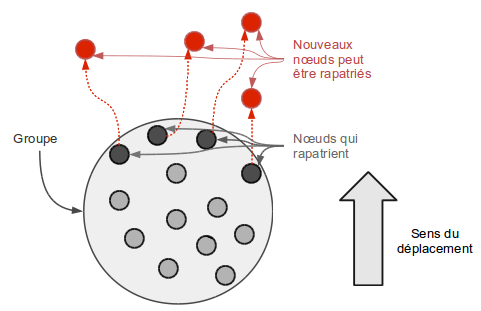
\includegraphics[scale=0.65]{./images/mouvgroup.png}
        \caption{Une piste pour les déplacements en groupe}
        \label{mouvgroup}
        \end{figure}

\newpage
\section{Autres}
Just Ro It !!!!


\newpage
\bibliographystyle{plain}
\bibliography{Biblio}


 

\end{document}
